\subsection{Corrected observable-data experiments}
\label{sec:observable_results}
The following analyses are post-hoc corrective reruns. The earlier comparator
grid used a pre-probe price as its first response coefficient; its method
rankings are withdrawn. The corrected inputs begin with the post-probe price,
$x_1$, and end at $x_{H+1}$. Failed fits and invalid endpoints count in the
attempted-panel denominator rather than being treated as covered intervals.
The earlier files remain in the archive; they are not pooled with these results.

\begin{table}[htbp]\centering\small
\caption{Assumption--implementation--evidence links for the corrected analyses.}
\label{tab:method_crosswalk}
\begin{tabular*}{\textwidth}{@{\extracolsep{\fill}}p{.25\textwidth}p{.34\textwidth}p{.32\textwidth}@{}}
\toprule
Method & Contract & Corrective artifact \\
\midrule
Recurrence LP & Theorem~\ref{thm:observable_stability}; Gaussian episode regression & \texttt{grid/results.json} \\
Conic relaxation & Known covariance: chi-square; estimated covariance: F. Numerical certification withheld. & \texttt{grid/}, \texttt{sweep\_known/}, \texttt{sweep\_estimated/} \\
Output-error & Single-rate local nonlinear fit; profile and sandwich intervals separately recorded & \texttt{grid/}, \texttt{diagnostic/} \\
Point/deconvolution & Constrained point heuristic or interval propagation & \texttt{grid/results.json} \\
Response-region pivot & Gaussian errors and independent Wishart covariance where estimated & \texttt{calibration/results.json} \\
\bottomrule\end{tabular*}
\par\smallskip\begin{minipage}{\textwidth}\footnotesize Paths are relative to \path{statistical_repair_20260926/verified/}. Source hashes, full per-panel observations, failure statuses and the repair protocol accompany these outputs. The separate audited-disclosure results in Section~\ref{sec:audited_inference} are not a matched estimator comparison on this grid.\end{minipage}
\end{table}


The corrected grid contains 600 independent panels within 120 fixed cells. The production design crosses $S\in\{.70,.82,1,1.03,1.18\}$,
slow rates $.002,.02,.10$, episode budgets $R=128,1024$, probe sizes $1,4$,
and horizons $H=24,64$, with five panels per cell. The aggregate rates are
descriptive averages over this fixed, heterogeneous design, not universal
performance guarantees or evidence that every cell is adequately powered.

\begin{table}[htbp]\centering\small
\caption{Corrective grid: containment and issued labels. All attempted panels are retained.}
\label{tab:comparator_comparison}
\begin{tabular*}{\textwidth}{@{\extracolsep{\fill}}lrrrrrr@{}}
\toprule
Method & Covered/$N$ & Issued/$N$ & Wrong & \shortstack{Wrong/$N$\\(\%)} & \shortstack{Wrong/issued\\(\%)} & Invalid \\
\midrule
Always abstain & 600/600 & 0/600 & 0 & 0.00 & -- & 0 \\
Recurrence LP & 597/600 & 0/600 & 0 & 0.00 & -- & 3 \\
Conic (numerical) & 600/600 & 0/600 & 0 & 0.00 & -- & 0 \\
Output-error & 193/600 & 438/600 & 204 & 34.00 & 46.58 & 31 \\
Interval deconvolution & 597/600 & 0/600 & 0 & 0.00 & -- & 3 \\
Constrained point fit & 228/600 & 483/600 & 165 & 27.50 & 34.16 & 0 \\
\bottomrule\end{tabular*}
\par\smallskip\begin{minipage}{\textwidth}\footnotesize Always abstain returns $[0,\infty)$ under the nonnegative model. Conic issued labels here are numerical candidates only: every certified label is withheld. Invalid or missing intervals are not covered. A zero wrong-label count with no issued labels is abstention, not successful discrimination. The point-fit interval has no nominal confidence guarantee.\end{minipage}
\end{table}

\begin{figure}[htbp]\centering
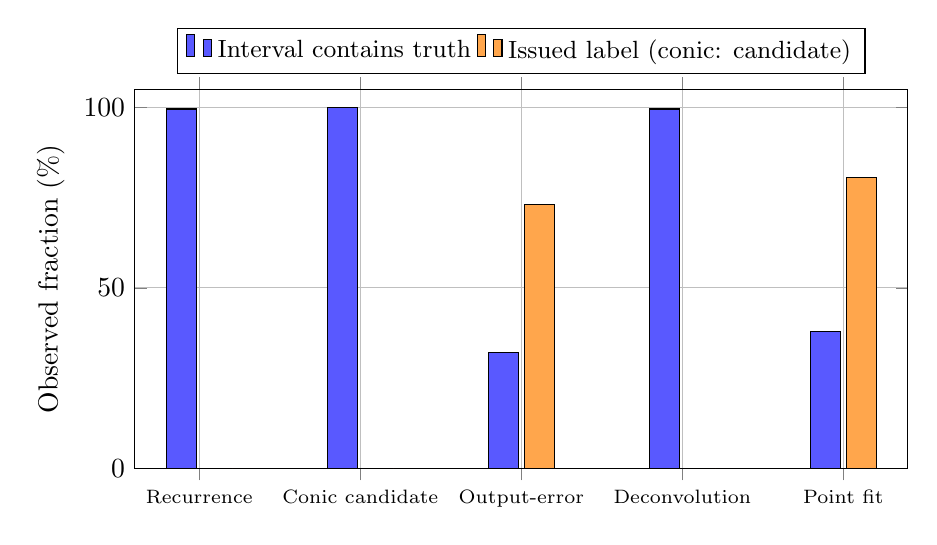
\begin{tikzpicture}\begin{axis}[
width=.94\textwidth,height=6.4cm,ybar,bar width=11pt,ymin=0,ymax=105,
ylabel={Observed fraction (\%)},xtick={1,2,3,4,5},
xticklabels={Recurrence,Conic candidate,Output-error,Deconvolution,Point fit},
x tick label style={font=\scriptsize},grid=major,
legend style={at={(.5,1.04)},anchor=south,legend columns=2,font=\small}]
\addplot[fill=blue!65,draw=black] coordinates {(1,99.500000) (2,100.000000) (3,32.166667) (4,99.500000) (5,38.000000)};
\addlegendentry{Interval contains truth}
\addplot[fill=orange!70,draw=black] coordinates {(1,0.000000) (2,0.000000) (3,73.000000) (4,0.000000) (5,80.500000)};
\addlegendentry{Issued label (conic: candidate)}
\end{axis}\end{tikzpicture}
\caption{Empirical containment and labeling on the corrected grid. These are
descriptive panel frequencies, not confidence bounds on performance. Conic
certification remains withheld; a candidate label is not a certified decision.
Audited-disclosure experiments use a different information contract and are
therefore not placed on this plot as a matched comparison.}
\label{fig:comparator_frontier}\end{figure}

\begin{table}[htbp]\centering\small
\caption{Interval availability and finite-width distributions on the corrected grid.}
\label{tab:corrective_widths}
\begin{tabular*}{\textwidth}{@{\extracolsep{\fill}}lrrrrr@{}}
\toprule
Method & Finite & Unbounded & Invalid & Finite mean & Finite $p_{90}$ \\
\midrule
Always abstain & 0 & 600 & 0 & -- & -- \\
Recurrence LP & 596 & 1 & 3 & 51.190 & 105.066 \\
Conic (numerical) & 472 & 128 & 0 & 125.639 & 245.685 \\
Output-error & 569 & 0 & 31 & 0.332 & 0.774 \\
Interval deconvolution & 596 & 1 & 3 & 127.918 & 294.159 \\
Constrained point fit & 600 & 0 & 0 & 0.137 & 0.182 \\
\bottomrule\end{tabular*}
\par\smallskip\begin{minipage}{\textwidth}\footnotesize Finite-width summaries condition on the finite count in that row. They are not unconditional mean widths when intervals are unbounded or invalid.\end{minipage}
\end{table}


In the grid, 472/600 panels have a cut-limit stop at one or both conic endpoints. A finite-cut outer candidate is not a converged second-order-cone optimum.


Output-error inference is unavailable on 31/600 panels. The conic routine records optimizer status, cut counts, residuals and both
objective corrections. Full outward rounding of all assembled constraints is
not established, so \texttt{certified=False} is returned even when a numerical
candidate separates $S$ from one. The exact-arithmetic outer-set theorem is
not a proof that floating-point endpoints have been certified.

\paragraph{Output-error benchmark and interval interpretation.}
The single-rate model fits $\theta=(a,\eta,Q,\kappa)$ by
\begin{equation}
 \min_\theta (\hat\beta-\beta(\theta))^\top W(\hat\beta-\beta(\theta))
       +\lambda(a^2+Q^2),\qquad \lambda=0.
 \label{eq:output_error_obj}
\end{equation}
The constraints are $0\le a\le.995$, $\underline\eta\le\eta\le1$,
$0\le Q\le4$, with $\kappa$ initialized at $\max(.001,\hat\beta_0)$
and bounded between $.1$ and $5$ times that initialization. Thus impact is
estimated, not supplied by the simulator oracle. The covariance inverse uses
the disclosed trace-scaled ridge $10^{-6}\operatorname{tr}(\widehat\Sigma)/(H+1)$.
With response Jacobian $J$, the reported covariance is the local
Gauss--Newton propagation
\[
 B J^\top W\widehat\Sigma WJ B,\qquad B=(J^\top WJ)^{-1}.
\]
This is not a general misspecification-robust variance formula for arbitrary
nonlinear models. Profile intervals use a local objective-increase threshold
and numerical nuisance minimization. The primary interval is the profile
interval when available; sandwich intervals are recorded separately. Neither
is a global profile-set certificate or a finite-sample guarantee. Failed
optimization, rank deficiency or an unavailable profile is retained as such,
without inventing a standard error or counting a fallback as valid inference.

\begin{table}[htbp]\centering\small
\caption{Response-region calibration, separate from structural interval optimization.}
\label{tab:response_pivot_calibration}
\begin{tabular*}{\textwidth}{@{\extracolsep{\fill}}llrrr@{}}
\toprule
Covariance & Pivot & Covered/draws & Coverage (\%) & \shortstack{Exact 99\%\\interval (\%)} \\
\midrule
Known & $\chi^2$ & 18975/20000 & 94.875 & [94.460, 95.268] \\
Estimated & $F$ & 19000/20000 & 95.000 & [94.590, 95.389] \\
\bottomrule\end{tabular*}
\par\smallskip\begin{minipage}{\textwidth}\footnotesize Dimension 25, episode-budget parameter 128; nominal coverage 95\%. Estimated mode draws an independent Wishart covariance. The fixed acceptance tolerance is one percentage point around nominal. Passing this check does not validate outward numerical constraint assembly.\end{minipage}
\end{table}

\paragraph{Known versus estimated covariance in the budget sweep.}
These experiments draw Gaussian response coefficients directly, not noisy
episode histories. Their covariance is either known exactly or estimated by
an independent Wishart draw. They are useful checks of covariance calibration
and numerical contraction, not evidence about fills, latency or exchange data.
The two modes share coefficient-noise draws; only their covariance treatment
differs. Each production cell has 20 draws and horizon $H=24$.

\begin{table}[htbp]\centering\small
\caption{Conic numerical endpoints at the first and last budget in each sweep.}
\label{tab:corrective_sweep}
\begin{tabular*}{\textwidth}{@{\extracolsep{\fill}}llrrrrr@{}}
\toprule
Covariance & $S$ & \shortstack{First\\width} & \shortstack{Last\\width} & \shortstack{Last\\covered/$N$} & \shortstack{Last\\candidates/$N$} & Wrong \\
\midrule
known & 0.60 & 7.306 & 2.343 & 20/20 & 0/20 & 0 \\
known & 0.82 & 11.203 & 4.856 & 20/20 & 0/20 & 0 \\
known & 1.25 & 17.151 & 11.198 & 20/20 & 20/20 & 0 \\
estimated & 0.60 & 7.701 & 2.344 & 20/20 & 0/20 & 0 \\
estimated & 0.82 & 12.316 & 4.857 & 20/20 & 0/20 & 0 \\
estimated & 1.25 & 18.186 & 11.199 & 20/20 & 20/20 & 0 \\
\bottomrule\end{tabular*}
\par\smallskip\begin{minipage}{\textwidth}\footnotesize Widths are unconditional means only when every interval is finite. Production budgets run from 128 to 32,768. All certified labels are withheld.\end{minipage}
\end{table}


Panels with a cut-limit stop at one or both endpoints are known: 300/300; estimated: 300/300. These are finite-cut outer approximations; the width curves do not demonstrate convergence to the exact conic optimum.

\begin{figure}[htbp]\centering
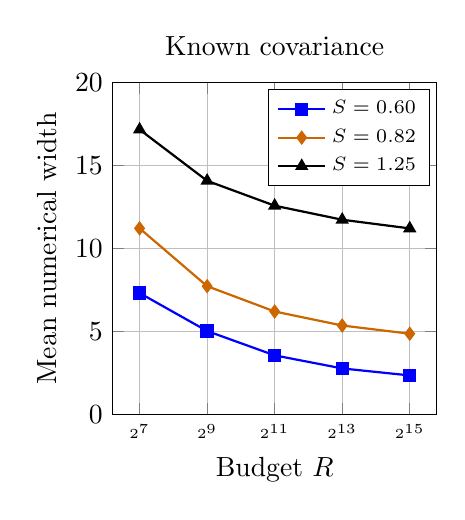
\begin{tikzpicture}\begin{axis}[width=.47\textwidth,height=5.8cm,xmode=log,log basis x=2,ymin=0,ymax=20.005,title={Known covariance},xlabel={Budget $R$},ylabel={Mean numerical width},xtick={128,512,2048,8192,32768},x tick label style={font=\tiny},grid=major,legend style={font=\scriptsize}]
\addplot[thick,mark=square*,blue] coordinates {(128,7.3064215) (512,5.0179377) (2048,3.5530190) (8192,2.7654996) (32768,2.3432830)};\addlegendentry{$S=0.60$}
\addplot[thick,mark=diamond*,orange!80!black] coordinates {(128,11.2027585) (512,7.7198119) (2048,6.1945459) (8192,5.3499027) (32768,4.8558387)};\addlegendentry{$S=0.82$}
\addplot[thick,mark=triangle*,black] coordinates {(128,17.1511538) (512,14.0646797) (2048,12.5665691) (8192,11.7215304) (32768,11.1983629)};\addlegendentry{$S=1.25$}
\end{axis}\end{tikzpicture}
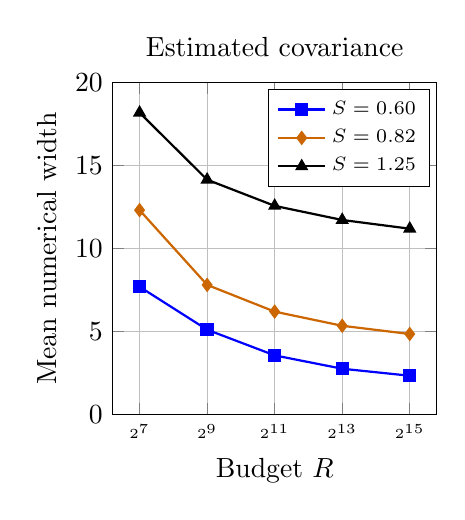
\begin{tikzpicture}\begin{axis}[width=.47\textwidth,height=5.8cm,xmode=log,log basis x=2,ymin=0,ymax=20.005,title={Estimated covariance},xlabel={Budget $R$},ylabel={Mean numerical width},xtick={128,512,2048,8192,32768},x tick label style={font=\tiny},grid=major,legend style={font=\scriptsize}]
\addplot[thick,mark=square*,blue] coordinates {(128,7.7014955) (512,5.1162723) (2048,3.5701028) (8192,2.7657969) (32768,2.3438433)};\addlegendentry{$S=0.60$}
\addplot[thick,mark=diamond*,orange!80!black] coordinates {(128,12.3162744) (512,7.8155581) (2048,6.2044836) (8192,5.3528670) (32768,4.8566271)};\addlegendentry{$S=0.82$}
\addplot[thick,mark=triangle*,black] coordinates {(128,18.1862491) (512,14.1514095) (2048,12.5751940) (8192,11.7246087) (32768,11.1992772)};\addlegendentry{$S=1.25$}
\end{axis}\end{tikzpicture}
\caption{Descriptive numerical interval widths under the two
covariance contracts, on common vertical scales. Each point averages a fixed
cell, not a confidence interval. Missing means indicate an invalid or unbounded
interval and are not imputed. Contraction is not certification or a universal
asymptotic claim.}\label{fig:conic_contraction}\end{figure}
\paragraph{Matched and misspecified output-error fits.}
C1/C3 are single deterministic cases, not repeated independent observations.
C2/C4 use independent Gaussian coefficient noise with known covariance, at
the same fixed horizon and noise scale. C1/C2 have one true rate; C3/C4 have
two rates but are fit by the same single-rate estimator. This design isolates
one form of structural mismatch; it does not establish an asymptotic bias
theorem or identify every reason for grid undercoverage. In particular, a
profile-interval result must not be relabeled as sandwich-interval coverage.

\begin{table}[htbp]\centering\small
\caption{Separate profile and sandwich diagnostics; true $S=.82$.}
\label{tab:output_error_diagnostic}
\begin{tabular*}{\textwidth}{@{\extracolsep{\fill}}lrrrrrr@{}}
\toprule
Case & Attempts & Mean $\hat S$ & Bias & \shortstack{Profile\\covered/valid} & \shortstack{Sandwich\\covered/valid} & Unavailable \\
\midrule
C1 & 1 & 0.8200 & 0.000000 & 1/1 & 1/1 & 0 \\
C2 & 100 & 0.8200 & -0.000037 & 91/100 & 93/100 & 0 \\
C3 & 1 & 0.7128 & -0.107218 & 0/1 & 0/1 & 0 \\
C4 & 100 & 0.7128 & -0.107205 & 0/100 & 0/100 & 0 \\
\bottomrule\end{tabular*}
\par\smallskip\begin{minipage}{\textwidth}\footnotesize Coverage denominators condition on an available interval of the named type; unavailable reports are counted separately. C1/C3 entries are deterministic containment only. The raw records also report optimizer failures, bound hits and interval fallbacks.\end{minipage}
\end{table}

\paragraph{What the corrected studies establish.}
The response-region probability calculation is a statement under its explicit
Gaussian sampling law. The comparator grid evaluates implemented methods,
including their numerical failures and modeling restrictions. Neither
experiment proves estimator superiority across information contracts, a
universal impossibility theorem, or real-market safety. The original
price-only primary experiment below remains a distinct dataset and is not
combined with this corrective grid.
